\chapter{Prototyping and Testing} \label{ch:prototyping}

\section{Prototyping Strategy}

The prototyping strategy was driven by a practical constraint: the production structure is to be fabricated in steel by Dawlance, but steel fabrication could not begin until the mechanical, electrical, and control designs were validated. A full-scale wooden prototype was therefore constructed to serve as a physical testbed for all subsystems prior to committing to steel fabrication. The wooden frame replicates the $4 \times 4 \times 2$\,m workspace envelope of the final system and provides mounting surfaces for the linear guide rails, servo motors, and end-effector assembly. While timber does not replicate the stiffness characteristics of steel, the prototype is sufficient for validating kinematic function, control logic, drive interfacing, and end-effector performance at low to moderate speeds.

Subsystem-level testing was performed incrementally: first individual components on a bench, then integrated onto the prototype frame. This approach allowed faults to be isolated to specific subsystems before full integration, reducing debugging complexity.


\section{Structural Assembly}

The wooden frame was assembled using outsourced carpentry to the workspace dimensions. GHR-30 series linear guide rails were installed on all three translational axes, with the X and Y axes using the four-block carriage configuration described in Chapter~4 to resist rolling and pitching moments. Cross-members were added between the parallel X-axis rails to maintain alignment under load.

The Z-axis rack-and-pinion mechanism was prototyped using 3D-printed spur gears (Module~2, 20~teeth) to validate mesh engagement and vertical travel before procurement of the final steel components. The 3D-printed mechanism demonstrated correct gear meshing and smooth vertical traversal, and the Z-axis was able to lift and lower a microwave shell smoothly under no-load and light-load conditions.

Figure~\ref{fig:prototype} shows the assembled prototype with all axes, servo motors, and the end-effector installed.

\begin{figure}[h]
    \centering
    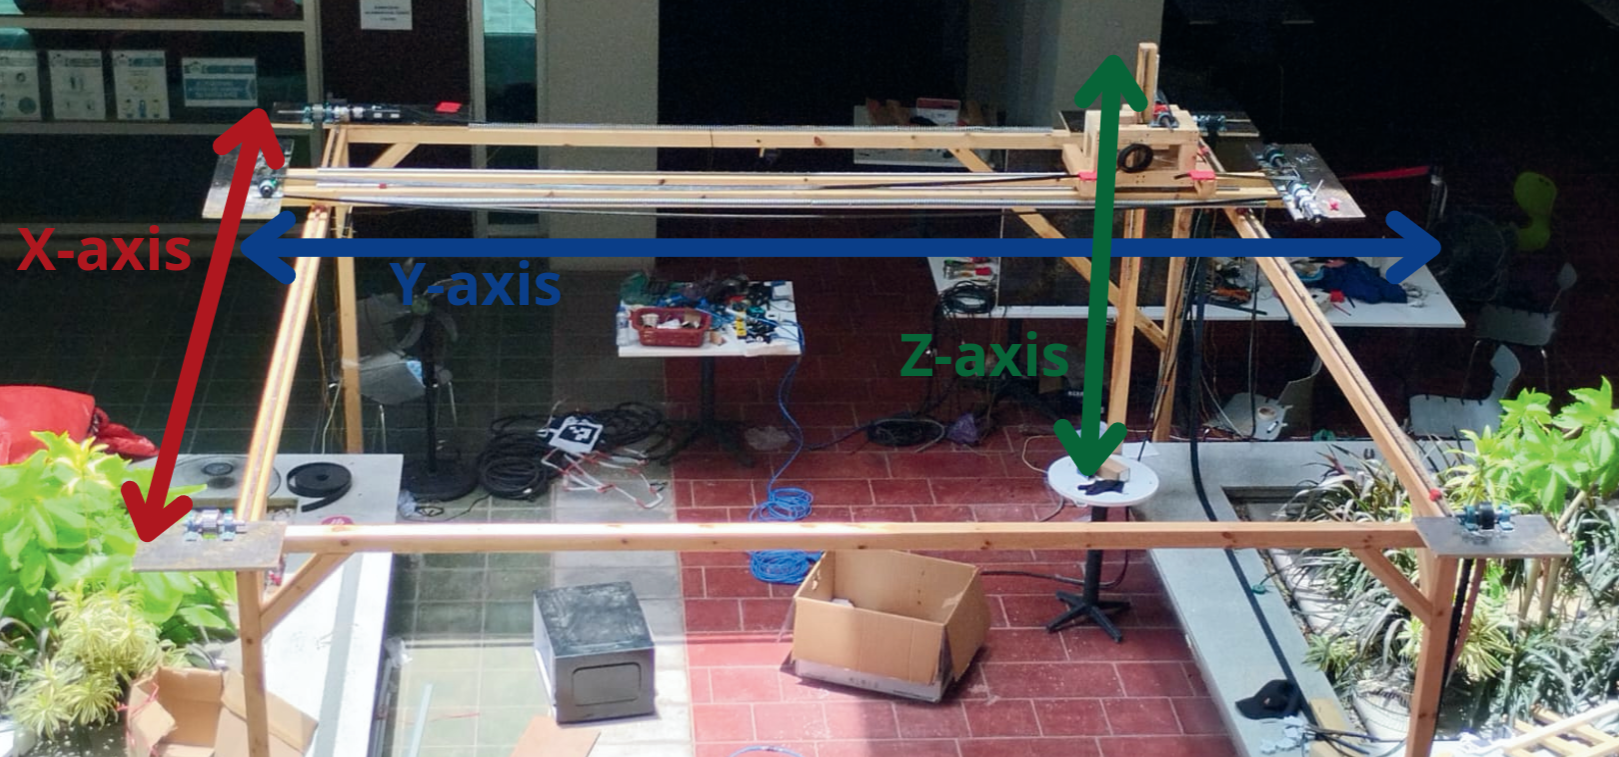
\includegraphics[width=0.9\textwidth]{figures/prototype_assembled.jpg} % UPDATE filename to match your actual image
    \caption{Full-scale wooden prototype with servo motors, linear guide rails, and end-effector assembled.}
    \label{fig:prototype}
\end{figure}


\section{Motor and Drive Validation}

All six Yaskawa Sigma-5 AC servo motors were mounted on the prototype frame and wired to their respective SGDV drives. Testing proceeded in two stages.

\subsection{Bench Testing}

Initial motor commissioning was performed on a bench using an Arduino Uno as a temporary pulse generator (Figure~9.1). The electronic gear ratio was configured on each drive by setting register Pn20E to 1,048,576 and Pn210 to 10,000, so that one full shaft revolution corresponds to exactly 10,000 command pulses. This was verified by issuing exactly 10,000 pulses and confirming a single revolution both visually on the motor shaft and through the pulse count displayed on the drive.

\subsection{Motion Profile Validation}

Once the motors were integrated onto the prototype, the S-curve motion profile generated by the STM32 firmware (Section~9.3) was compared against direct step commands without acceleration shaping. With the S-curve profile active, axis motion was noticeably smoother, with no audible vibration or mechanical shock at the start and end of travel. Without the S-curve --- that is, with an abrupt step input --- the motors exhibited visible jerk at the transitions between stationary and moving states. No drive faults (such as the A.d00 following error) were triggered during S-curve operation.

The electromagnetic brakes on all axes were tested by enabling and disabling the 24\,V brake supply while the axis was stationary under load. The brakes engaged and held position reliably in all tests, confirming their function as a safety mechanism against backdrive on the Z-axis in the event of power loss.


\section{End-Effector Validation}

The vacuum end-effector was assembled on the prototype, comprising two 125\,mm and four 50\,mm FESTO bellows suction cups mounted on an aluminium extrusion frame, connected via T-connectors and 8\,mm push-in fittings to the FESTO VN-14 vacuum generator.

\subsection{Static Lift Test}

A static lift test was conducted with the suction cups in isolation (not mounted on the prototype frame) to determine the maximum holding capacity of the vacuum system. Steel plates from a standard weight set were incrementally loaded onto a flat surface gripped by the suction cup array. The system successfully held 40\,kg without detachment, meeting the design payload specification. Teflon tape was applied to all threaded NPT connections to minimise vacuum leakage, though minor leakage at some interfaces was observed and is noted as a limitation in Section~\ref{sec:limitations}.

\subsection{Integrated Pick-and-Move Test}

With the end-effector mounted on the prototype, pick-and-move operations were performed on a Dawlance microwave unit. The suction cups were engaged on the top surface of the microwave through its plastic wrapping, the Z-axis lifted the unit, and the X and Y axes translated it across the workspace under manual teleoperation via the WASD command interface. The microwave was then lowered and released by de-energising the solenoid valve.

This operation was performed repeatedly over extended periods during the project showcase at Habib University, with the system running for over one hour of cumulative operation without a single grip failure or observable product damage. The microwave was moved across the full X--Y workspace envelope during these demonstrations. However, traversal speeds were limited to avoid exciting resonances in the wooden frame, so these tests do not validate the cycle time specification.

No damage to the microwave shell or plastic wrapping was observed after repeated handling. The bellows-type suction cups conformed to the surface without requiring precise alignment, confirming their suitability for the non-uniform top surfaces of Dawlance microwave models.


\section{Computer Vision Validation}

Two vision pipelines were developed and tested during the project.

\subsection{Classical Pipeline}

The initial pipeline, described in Chapter~10, uses HSV colour-space thresholding, morphological filtering, and contour extraction with minimum-area rectangle fitting. This pipeline was tested on a real Dawlance microwave and its corresponding box. Orientation estimation was accurate to within half a degree. However, position estimation exhibited errors caused by the open flaps of the box and the protruding edges of the microwave, which distorted the contour shape and shifted the computed centre.

\subsection{YOLO-Based Pipeline}

A YOLO26-Nano (YOLO26n) model was trained on a custom dataset of manually annotated images of a Dawlance microwave and its box, photographed in various positions and orientations. YOLO26n was selected for its low inference latency, which is advantageous for real-time control loops. The model demonstrated reliable detection and keypoint localisation for both object classes. However, the Euclidean distance estimate from the camera origin fluctuated between successive frames, indicating instability in the pose estimation that would require temporal filtering (e.g., a moving average or Kalman filter) before use in closed-loop control. Additionally, the model has been trained on a single microwave model and box type; generalisation to Dawlance's full product range would require an expanded training dataset.

\subsection{GDino + SAM2 Pipeline}

A third pipeline using Grounding DINO for open-vocabulary detection, SAM2 for pixel-level segmentation, and PnP homography for pose mapping was developed and tested with the AR0234 global shutter camera. This pipeline achieved a position error of approximately 5\% relative to the object's distance from the camera origin, which, as discussed in Section~\ref{sec:limitations}, exceeds the $<1$\,cm accuracy specification and is attributed to camera calibration. Yaw estimation was qualitatively correct. This pipeline has the advantage of requiring no training data, making it immediately applicable to new microwave models.


\section{Control System Validation}

\subsection{Homing Routine}

A homing routine was implemented and validated on the X and Y axes of the wooden prototype. Each axis drives toward its limit switch at a moderate speed until the switch triggers, then reverses slowly until the switch releases. The final position is registered as the axis origin, and all subsequent motion commands are referenced to this coordinate. The routine executed reliably across multiple power cycles, confirming repeatable initialisation.

\subsection{Teleoperation Interface}

The Python CLI (Chapter~\ref{ch:interface}) was validated as the primary control interface during all integrated testing. Commands entered via the keyboard were serialised to JSON, transmitted to the STM32 over UART/USB, parsed, and executed as motor trajectories. The WASD teleoperation mode was used extensively during the showcase demonstrations, with the operator controlling X and Y translation in real time while the vacuum system held the microwave. No communication faults or command parsing errors were observed.

\subsection{Simulation}

The PyBullet simulation environment was used to validate the finite state machine logic and image-based visual servoing (IBVS) control law prior to hardware integration. The simulation confirmed that the IBVS controller could converge on a target object with randomised initial position and yaw, providing confidence in the control architecture before deployment on the physical prototype.


\section{Summary of Validation Status}

Table~\ref{tab:validation_summary} summarises the current validation status of each design specification against the metrics defined in Section~2.5.

\begin{table}[h]
\centering
\caption{Validation status of key design specifications.}
\label{tab:validation_summary}
\begin{tabularx}{\textwidth}{l l l X}
\toprule
\textbf{Specification} & \textbf{Target} & \textbf{Status} & \textbf{Notes} \\
\midrule
Payload capacity & 40\,kg & Validated & Static lift test with weight plates; sustained grip during pick-and-move. \\
Positional accuracy & $<1$\,cm & Partially validated & Vision pipeline achieves $\sim$5\% error (calibration-limited); motor positioning verified via electronic gear ratio. \\
Positional repeatability & $\pm\,0.5$\,cm & Not yet validated & Requires formal measurement campaign on steel structure. \\
Orientation accuracy & $\pm\,1.0^{\circ}$ & Partially validated & Classical CV pipeline accurate to $0.5^{\circ}$; YOLO pipeline exhibits frame-to-frame fluctuation. \\
Cycle time & $\leq 30$\,s & Not yet validated & Motor sizing confirms feasibility; prototype limited to low speed due to wooden frame resonance. \\
Pick reliability & $\geq 99/100$ & Preliminary & No grip failures in $>$1\,hr of continuous operation; formal 100-cycle trial pending. \\
Place reliability & $\geq 99/100$ & Not yet validated & Placement at representative speed and accuracy requires steel structure. \\
Yaw axis & $\pm\,1.0^{\circ}$ & Component-level & Motor, gearbox, and bearings validated individually; not integrated on prototype. \\
Budget & $\leq$ Rs\,1.8M & Met & BOM total Rs\,1,779,400 including 25\% contingency. \\
\bottomrule
\end{tabularx}
\end{table}

The table reflects that the prototype successfully validated the core functional subsystems --- structural assembly, motor actuation, vacuum gripping, computer vision detection, and control communication --- while the quantitative performance specifications (accuracy, repeatability, cycle time) require the rigidity of the production steel structure for formal measurement. The commissioning tests recommended in Section~\ref{sec:near_term} are designed to close these remaining validation gaps.